\documentclass{article}
\usepackage[utf8]{inputenc}
\usepackage{fullpage}
\usepackage{url}
\usepackage[parfill]{parskip}
\usepackage{graphicx}
\usepackage{amsmath}
\usepackage{algorithm}
\usepackage{algpseudocode}

\title{\Large \textbf{Attacking AES using CPA}\\
Embedded Security Project
}
\author{
{\rm Andreas L\"{o}fwenmark and Chih-Yuan Lin}\\
Department of Computer and Information Science\\
Linköping University\\
Sweden
%\and
%{\rm Chih-Yuan Lin}\\
%Department of Computer and Information Science\\
%Linköping University\\
%Sweden
}

\begin{document}
%\date{}

\maketitle

\section{Introduction}
This report summarizes the project work of the Embedded Security course. Our assignment was to implement a differential power analysis (DPA) side-channel attack on the Advanced Encryption Standard (AES) algorithm using correlation power analysis (CPA).

%\section{Assignment}

\section{Method}
The method we used for performing the DPA attack is based on the strategy outlined by Mangard et al.~\cite[Ch.\ 6]{paa2007}. It consists of the following steps:
\begin{enumerate}
\item Choosing an intermediate result of the executed algorithm.
\item Measuring the power consumption.
\item Calculating hypothetical intermediate values.
\item Mapping intermediate values to power consumption values.
\item Comparing the hypothetical power consumption values with power traces.
\end{enumerate}
In this project we chose the S-box outputs in the first round, since the generation of first round result is simple and not error-prone given the plaintext. We did not need to perform any power consumption measurements as power traces were given to us\footnote{\url{https://www.assembla.com/spaces/chipwhisperer/wiki/Example_Captures}}. To map the intermediate values to power consumption values we used the Hamming Weight model. We used correlation power analysis to compare our calculated hypothetical power consumption values with the provided power traces. The correlation is calculated using Pearson's correlation coefficient (Equation~\ref{eq:corr}). The intuition is that a correct key hypothesis results in a good correlation between the model and real power consumption. 

\begin{equation}
  \rho_{X,Y}=\frac{cov(X, Y)}{\sigma_X\sigma_Y}=\frac{E\left[(X-\mu_X)(Y-\mu_Y)\right]}{\sqrt{E\left[(X-\mu_X)^2\right]}\sqrt{E\left[(Y-\mu_Y)^2\right]}}
  \label{eq:corr}
\end{equation}

\subsection{Simulation}
Before starting real CPA attack, we ran the simulation attack first. The purpose of running simulation attack is to verify our implementation of given intermediate value and power model with a known effective single trace. After verification, we then extended our work to real multiple traces.

The Simulation attack is conducted with the known key 198. Figure~\ref{fig:bad_sim} shows the simulation result when the S-box of the encryption algorithm is not correctly implemented. The incorrect implementation is losing an important property of S-box, the non-linearity. Compare to the correct and final version in Figure~\ref{fig:good_sim}. Loss of non-linearity makes the correlation of other keys higher, though the peak is still in key 198. Therefore, we assume the result of CPA should display a characteristic like Figure~\ref{fig:good_sim}.

\begin{figure*}[ht]
  \centering
  \begin{minipage}[b]{0.45\linewidth}
    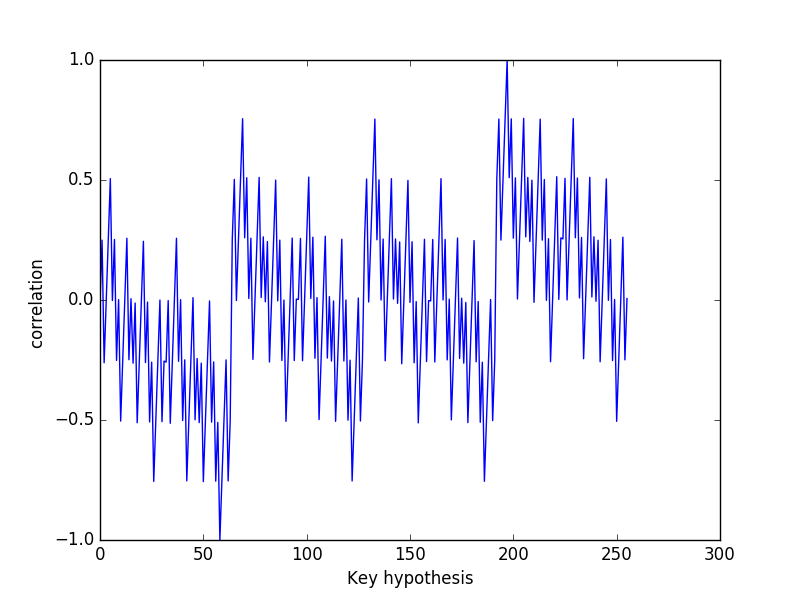
\includegraphics[scale=0.35]{bad_simulation.png}
    \caption{Bad simulation}
    \label{fig:bad_sim}
  \end{minipage}
  \quad
  \begin{minipage}[b]{0.45\linewidth}
    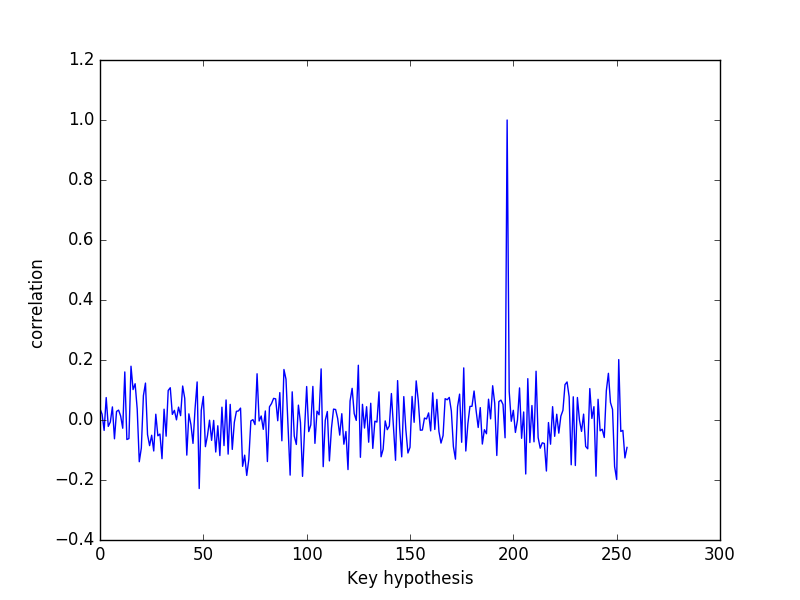
\includegraphics[scale=0.35]{good_simulation.png}
    \caption{Good simulation}
    \label{fig:good_sim}
  \end{minipage}
\end{figure*}

\subsection{Implementation}
The Python implementation for the CPA attack can be found on GitHub\footnote{\url{https://github.com/hwdev/Embedded-Security}}. The program takes one argument, the base name (\{base\}) of the power traces. A number of files are expected to exist in NumPy\footnote{\url{http://www.numpy.org}} (.npy) format, \{base\}\_traces.npy, \{base\}\_textin.npy and \{base\}\_knownkey.npy.

The pseudo code of the main function is shown in Algorithm~\ref{alg:main} and the key guessing function is shown in Algorithm~\ref{alg:guess}.

\begin{algorithm}[H]
  \caption{Pseudo Code for CPA attack}
  \label{alg:main}
  \begin{algorithmic}[1]
    \Procedure{CPA}{}
    \State Load power $traces$, $plaintext$ and $knownkey$
    \For{each byte $i$ in AES key}
    \State \Call{GuessKeyByte}{$i$}
    \State Print guessed key
    \EndFor
    \State Print $knownkey$
    \EndProcedure
  \end{algorithmic}
\end{algorithm}

\begin{algorithm}[H]
  \caption{Pseudo Code for guessing a key byte}
  \label{alg:guess}
  \begin{algorithmic}[1]
    \Function{GuessKeyByte}{$byteNum$}
    \For{$keyGuess$ in range(0, 256)}
    \ForAll{$traces$}
    \State Get S-box output using plaintext[$byteNum$] and $keyGuess$
    \State Calculate hypothetical power consumption (Hamming Weight) on S-box output
    \EndFor
    \ForAll{$traces$}
    \State Calculate correlation coefficients using Equation~\ref{eq:corr}
    \EndFor
    \EndFor
    \State\Return index of maximum correlation (our guessed key)
    \EndFunction
  \end{algorithmic}
\end{algorithm}

\section{Results}
To test our implementation, we downloaded the file avr\_aes128\_10000.zip\footnote{\url{https://www.assembla.com/spaces/chipwhisperer/documents/c9YGi-G5ir44xdacwqjQXA/download/c9YGi-G5ir44xdacwqjQXA}} containing 10,000 traces with 3,000 point in each trace.

Figure~\ref{fig:key_1} and Figure~\ref{fig:key_2} show the correlation for key byte 1 and 2, they both show a characteristic similar to Figure~\ref{fig:good_sim} giving us confidence that we have a good implementation using multiple traces and also that we have found the correct key byte.

Our CPA implementation successfully identified the correct key in about 40 minutes.

\begin{figure*}[ht]
  \centering
  \begin{minipage}[b]{0.45\linewidth}
    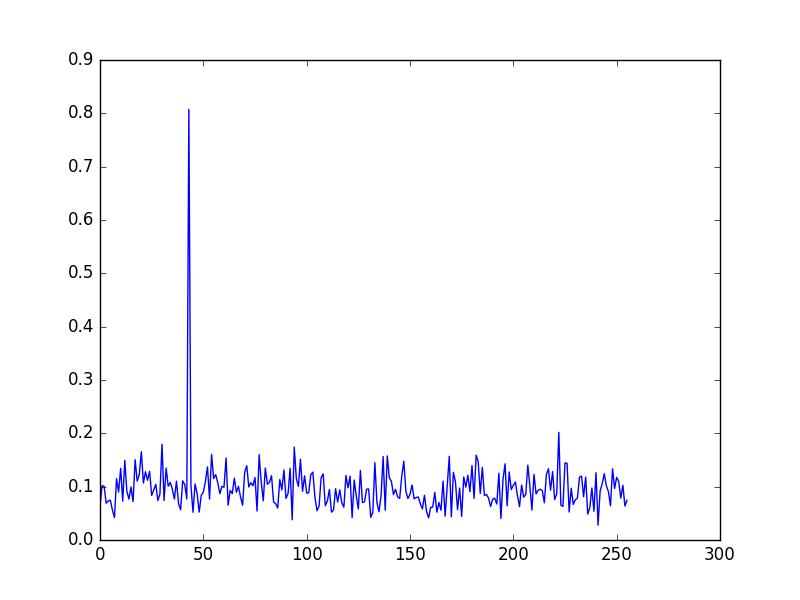
\includegraphics[scale=0.35]{figure_1_1.png}
    \caption{AES key hypothesis, byte 1}
    \label{fig:key_1}
  \end{minipage}
  \quad
  \begin{minipage}[b]{0.45\linewidth}
    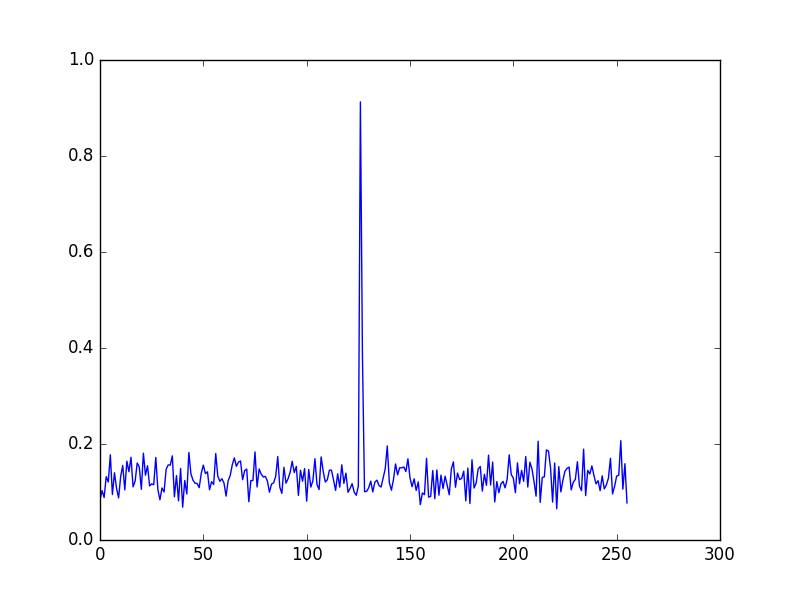
\includegraphics[scale=0.35]{figure_1_2.png}
    \caption{AES key hypothesis, byte 2}
    \label{fig:key_2}
  \end{minipage}
\end{figure*}

\bibliographystyle{unsrt}
\bibliography{refs}

\end{document}
